\documentclass[tikz]{standalone}
\usepackage{tikz, mathrsfs}
\usetikzlibrary{arrows, backgrounds}

\definecolor{vermelho}{RGB}{216,140,154}
\definecolor{verde}{RGB}{153,193,185}
\definecolor{azul}{RGB}{142,125,190}
\definecolor{amarelo}{RGB}{203,200,123}

\begin{document}

\def \dx {.25}
\def \dy {.6}
\def \sepx {.35}
\begin{tikzpicture}[scale=2.3, auto, swap]
    \node at (-.6,.72) {(a)};

    % reservoirs
    \fill[rounded corners=1pt, fill=azul] (\sepx, 0) rectangle ++(\dx, \dy) {};
    \fill[rounded corners=1pt, fill=verde] (-\sepx, 0) rectangle ++(-\dx, \dy) {};
    \fill[rounded corners=1pt, fill=vermelho] (\sepx, -1) rectangle ++(\dx, \dy) {};
    \fill[rounded corners=1pt, fill=amarelo] (-\sepx, -1) rectangle ++(-\dx, \dy) {};
    \node at (\sepx+0.5*\dx,.4) {T};
    \node at (\sepx+0.5*\dx,.2) {\(\mu_2\)};
    \node at (-\sepx-0.5*\dx,.4) {T};
    \node at (-\sepx-0.5*\dx,.2) {\(\mu_1\)};
    \node at (\sepx+0.5*\dx,.4-1) {T};
    \node at (\sepx+0.5*\dx,.2-1) {\(\mu_4\)};
    \node at (-\sepx-0.5*\dx,.4-1) {T};
    \node at (-\sepx-0.5*\dx,.2-1) {\(\mu_3\)};

    % energy levels
    \draw[thick] (-\dx/2,\dy/2) -- (\dx/2,\dy/2);
    \draw[thick] (-\dx/2,\dy/2-1) -- (\dx/2,\dy/2-1);

    % quantum dots
    \draw[fill=white, draw=black] (0,\dy/2+.13) circle (.1);
    \node at (0,\dy/2+.13) {$\epsilon_u$};
    \draw[fill=white, draw=black] (0,\dy/2+.13-1) circle (.1);
    \node at (0,\dy/2+.13-1) {$\epsilon_d$};
    \usetikzlibrary{decorations.pathmorphing}
    \path[style={decorate, decoration=snake}, draw=black] (0,\dy/2+.13-.1) -- node[right,midway] {$\Delta \epsilon$} (0,\dy/2+.13-1+.1);
    
    % exchanges
    \draw [->,azul] (\sepx/2,\dy/2+.13) to [out=30,in=150] (\sepx/2+.15,\dy/2+.13);
    \draw [<-,azul] (\sepx/2,\dy/2+.13-.05) to [out=30,in=150] (\sepx/2+.15,\dy/2+.13-.05);
    \draw [->,verde] (-\sepx/2,\dy/2+.13) to [out=150,in=30] (-\sepx/2-.15,\dy/2+.13);
    \draw [<-,verde] (-\sepx/2,\dy/2+.13-.05) to [out=150,in=30] (-\sepx/2-.15,\dy/2+.13-.05);

    \draw [->,vermelho] (\sepx/2,\dy/2+.13-1) to [out=30,in=150] (\sepx/2+.15,\dy/2+.13-1);
    \draw [<-,vermelho] (\sepx/2,\dy/2+.13-.05-1) to [out=30,in=150] (\sepx/2+.15,\dy/2+.13-.05-1);
    \draw [->,amarelo] (-\sepx/2,\dy/2+.13-1) to [out=150,in=30] (-\sepx/2-.15,\dy/2+.13-1);
    \draw [<-,amarelo] (-\sepx/2,\dy/2+.13-.05-1) to [out=150,in=30] (-\sepx/2-.15,\dy/2+.13-.05-1);

    \node at (.8,.72) {(b)};
    \begin{scope}[xscale=.9,shift={(1,-.7)}]
       \def \L {1};
        \def \ang {25};
        \node (00) at (0,0) {00};
        \node (01) at (0,\L) {01};
        \node (10) at (\L,0) {10};
        \node (11) at (\L,\L) {11};
        
        \path (00) edge [bend left=\ang, thick, verde!90!black] node [left, midway] {1} (01);
        \path (00) edge [bend right=\ang, thick, azul!90!black] node [right, midway] {2} (01);
        \path (10) edge [bend left=\ang, thick, azul!90!black] node [left, midway] {2} (11);
        \path (10) edge [bend right=\ang, thick, verde!90!black] node [right, midway] {1} (11);

        \path (01) edge [bend left=\ang, thick, amarelo!90!black] node [above, midway] {3} (11);
        \path (01) edge [bend right=\ang, thick, vermelho!90!black] node [below, midway] {4} (11);
        \path (00) edge [bend left=\ang, thick, vermelho!90!black] node [above, midway] {4} (10);
        \path (00) edge [bend right=\ang, thick, amarelo!90!black] node [below, midway] {3} (10);

        \node at (0, \L/2) {$A_{12}$};
        \node at (\L, \L/2) {$A_{12}$};
        \node at (\L/2, 0) {$A_{34}$};
        \node at (\L/2, \L) {$A_{34}$};
        
    \end{scope}

    \node at (3,-.27) {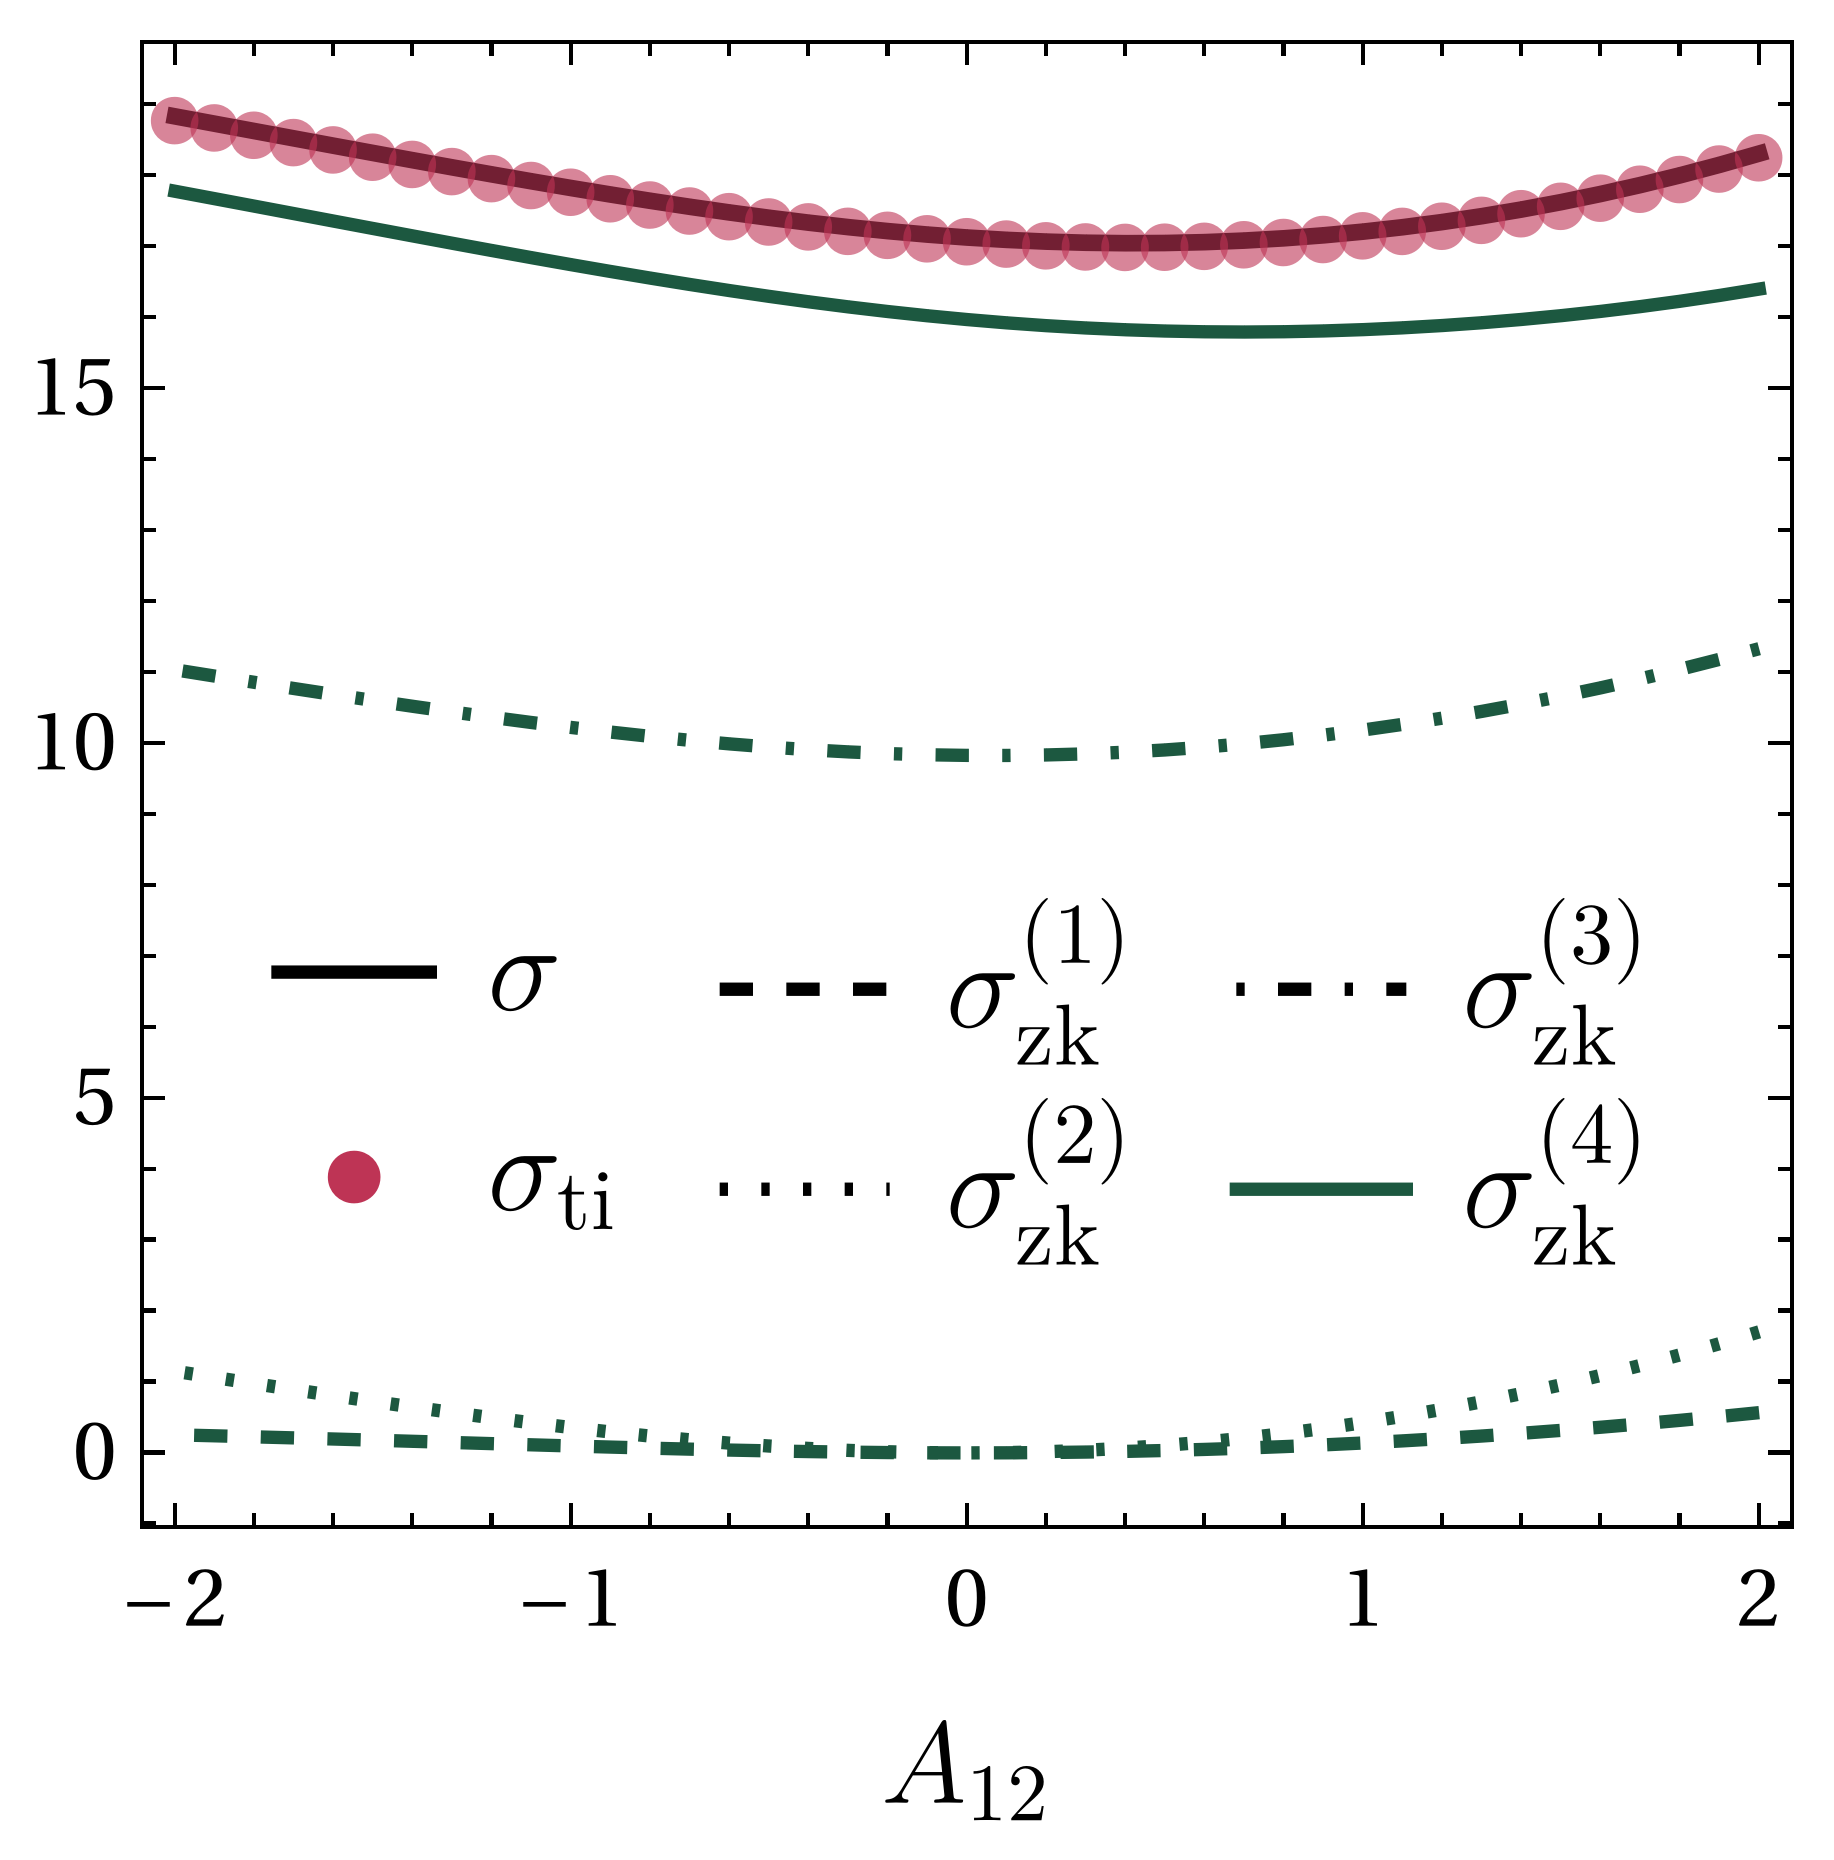
\includegraphics[width=0.35\textwidth]{plot_DD_EPR.png}};
    \node at (2.1,.72) {(c)};
    
    \node at (4.86,-.27) {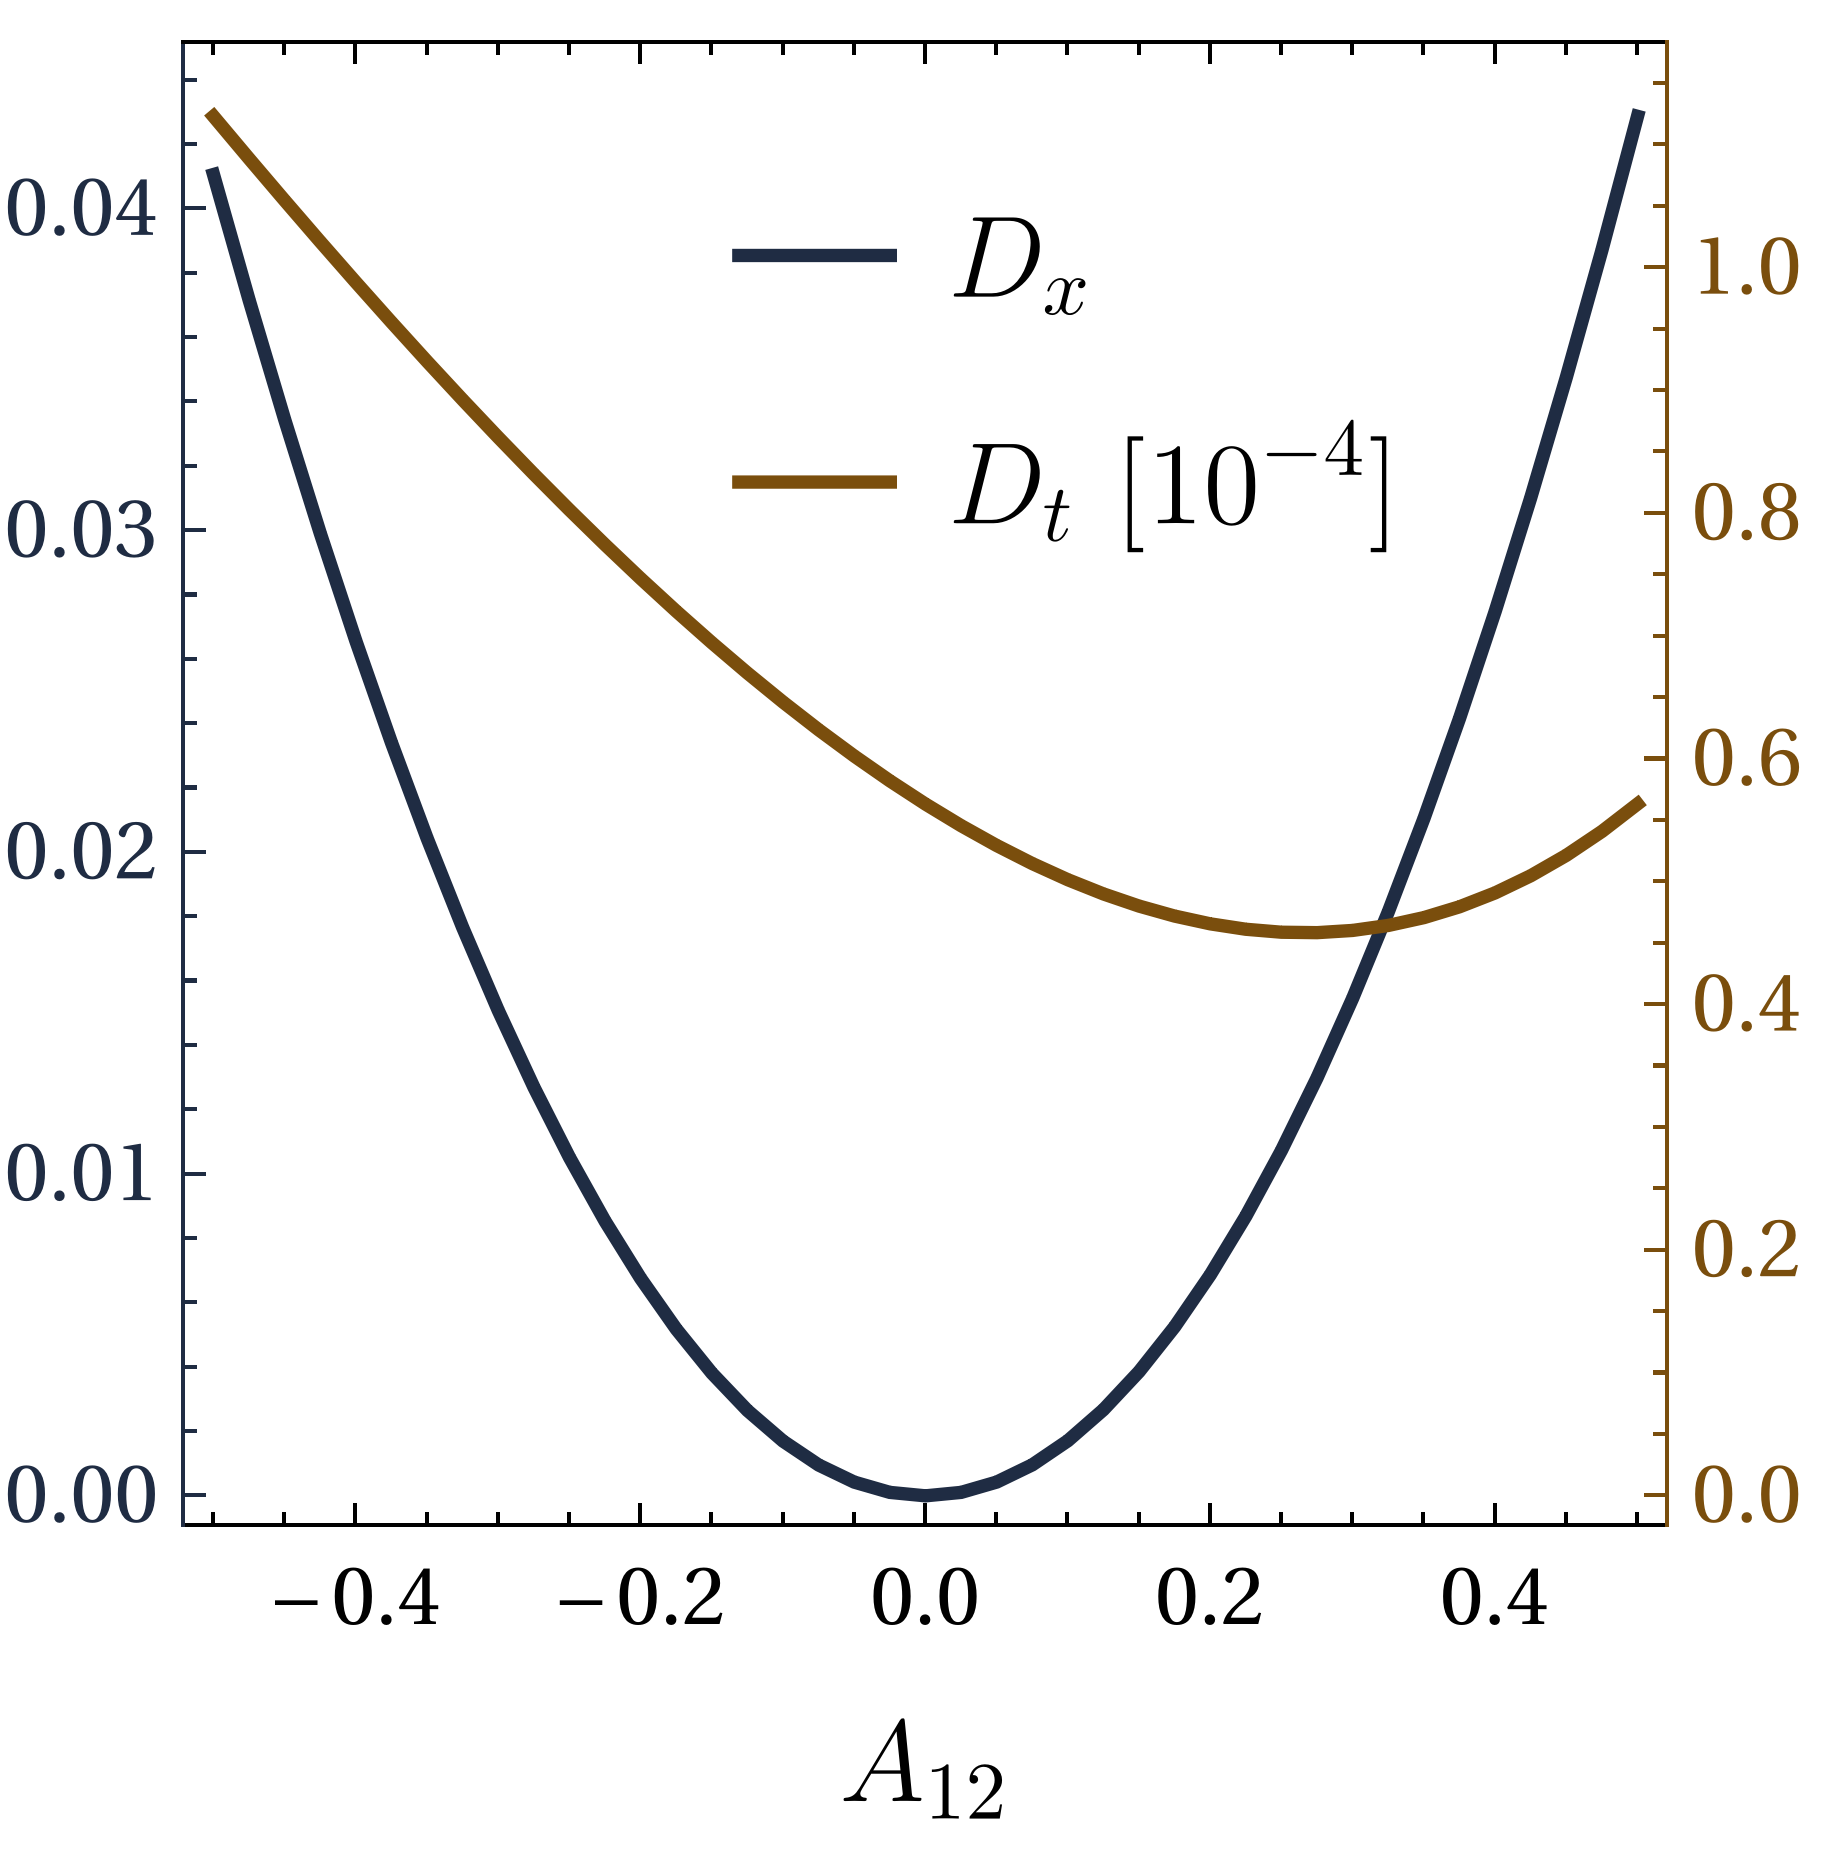
\includegraphics[width=0.35\textwidth]{plot_DD_Dxt.png}};
    \node at (4,.72) {(d)};
    
\end{tikzpicture}


\end{document}
